\label{sec:charakterbogen}\begin{quote}
    Ach ich darf mein Leben gar nicht für die Punkte opfern?
\end{quote}
\subsection{Allgemeine Daten}

Hierbei sei erst einmal gesagt, dass das endgültige Layout des Charakterbogens noch nicht fertig ist (und ich gerne Designs/Zeichnungen von euch darin einbaue um das Ganze aufzuhübschen \Laughey) und ihr deswegen hier nur pragmatische Darstellungen der jeweiligen Sektion seht, die nur aus semantischer Sicht so übernommen werden.

\index{Punkte}Wichtig ist, dass es diesmal \index{Punkte!Spezifisch (\SP)}spezifische (\SP{}) und \index{Punkte!Global/Magisch (\GP)}globale (\GP{}) Punkte gibt. \SP{} sind an eine Fertigkeiten-Gruppe gebunden. \SP{} können \(4:1\) in \GP{} umgewandelt und damit auch in anderen Gruppen eingesetzt werden (\GP{} sind allerdings nicht mehr Wert, die einzige Ausnahme hiervon ist die Magie\ldots).% TODO: link Magie

\paragraph{Allgemeine Metadaten}
\label{par:charMeta}\begin{sccenter}
    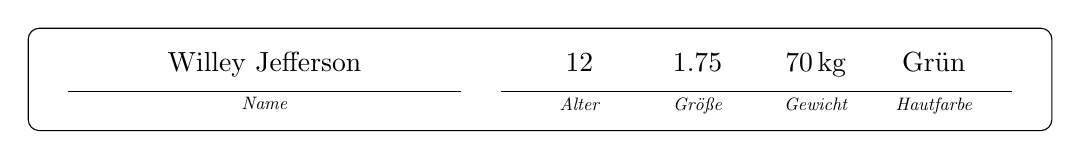
\begin{tikzpicture}[lc/.style={below,scale=0.65,font=\itshape}]
        \draw[rounded corners] (0,0) rectangle ++(13,1.3);
        \draw (0.5,0.5) -- ++(5,0) node[lc,midway] {Name} node[above,midway] {\strut{Willey Jefferson}};
        \draw (6,0.5) -- ++(6.5,0);
        \foreach[count=\i] \a/\b in {12/Alter,1.75/Größe,70\,kg/Gewicht,Grün/Hautfarbe} {
            \node[lc] at(7+1.5*\i-1.5,0.5) {\b}; 
            \node[above] at(7+1.5*\i-1.5,0.5) {\strut\a}; 
        }
    \end{tikzpicture}
\end{sccenter}
Die Daten, die dort eingetragen werden sollen, sollten ohne große Erklärung funktionieren. Deswegen hopp hopp, und weiter geht die Reise\ldots

\paragraph{Die Lebensversicherung}
\begin{wrapfigure}{l}{0.45\linewidth}
    \centering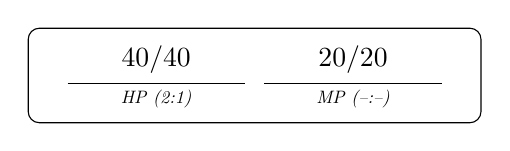
\begin{tikzpicture}[lc/.style={below,scale=0.65,font=\itshape}]
        \draw[rounded corners] (0,0) rectangle ++(5.75,1.2);
        \draw (0.5,0.5) -- ++(2.25,0) node[lc,midway] {HP (2:1)} node[above,midway] {40/{\smaller40}};
        \draw (3,0.5) -- ++(2.25,0) node[lc,midway] {MP (--:--)} node[above,midway] {20/{\smaller20}};
    \end{tikzpicture}
\end{wrapfigure}
Erstmal zu den \imp{Lebenspunkten (HP)}: 
Ihr startet mit 40, was nach verhältnismäßig wenig klingt aber schon ganz ordentlich ist im Verhältnis zum allgemeinen Schadenssystem. % TODO: LinK
Die Kosten für Leben betragen \(2:1\) und können aus allen anderen Gruppen zusammengespart werden. Der Verkaufspreis ist invertiert, ein Lebenspunkt liefert also zwei Fertigkeitenpunkte (\SP).
Die Lebenspunkte dürfen durch das verkaufen nicht auf oder unter Null gesetzt werden. Weniger Lebenspunkte werden aber auch hart bestraft\ldots

\subsection{Ausrüstung}

\subsection{Inventar}

\subsection{Fertigkeiten}